\section{Sugihara Causality}
The concepts of abstract correspondence, correlation and interpreting causation has been discussed in philosophical literature at least as early as Berkley's and Locke's arguments on human perception \cite{Locke1841} \cite{Berkeley1874}. Until now, the debate focused on what constitutes a causative effect and how such an effect might be discerned. From philosophy, the debate has moved to empirical science, where different models of causality have been proposed, none of which has been declared the true standard. Causality is often mistaken for correlation because the relationship between the two is not always clear. For example, falling down the stairs could be correlated with breaking a limb, but is falling down the stairs caused by breaking a limb, or is breaking a limb caused by falling down the stairs? One might argue that a person wouldn't break a limb without falling down the stairs, but what if a limb was stressed enough that it broke while a person was normally walking down the stairs, causing the person to lose control of their leg and therefor fall? In this sense, causality is a murky subject that is often considered to be highly subjective and at times nondetachable from the context of the situation. With that being said, there have been many attempts to address the concept of causality in mathematics in the form of the causality of continuous signals on one another. For example, if one could attain the stock prices for hot dogs and hot dogs buns, one would be able to hypothetically see a correlation between the sales of hot dogs and hot dog buns. It is also clear that one can describe a logical causation between the two stock prices, since the products are complementary to one another: if the price for one goes down, the price for the other goes down as well. For the case when substantial fluctuations happen in the stock price for both products, how would one determine which product caused the change in the price of the other? Surely the price drop was caused by \textit{something}, so which of the products caused the other? This is where causality models come into play---this is an example of the use of causality models in the field of Economy.

A particular causality model, Granger Causality (GC), has been widely used in application in the econometric fields \cite{Granger1969}, and has been the de facto model when causality is concerned. The way Granger Causality works is beyond the scope of this paper, but suffice it to say that Granger Causality behaves best in linear, stochastic systems. However, this causality model carries its own limitations, as, even with extensions to non-linear systems, it has generally not been seen capable of inferring causality in deterministic systems where feedback loops and nonlinearity are a defining feature. New models of causality have been introduced to attempt to go beyond these limitations. Dynamic Bayesian Networks and, more recently, the Convergent Cross Mapping (CCM) are some such models. The CCM model, also called Sugihara Causality model, relies on the convergence of distance of nearest neighbors in the shadow manifold of pairs of variables \cite{Sugihara2012}. To understand what all this means, we must first discuss manifolds (also called attractors).

\subsection{Manifolds}
Given three time series, a manifold of those three series is a new, three-dimensional representation of the state of the three variables at each time point. If the time series are somehow related to a specific concept, then this concept is called a \textit{system}, and the manifold then represents the state progression of the system. To illustrate this, a common example is used, namely the Lorenz Attractor. The Lorenz system is made up of three time series that are governed by the following differential equations

\begin{align}
\frac{\partial x}{\partial t} &= \sigma(y-x) \\
\frac{\partial y}{\partial t} &= x(\rho-z) - y \\
\frac{\partial z}{\partial t} &= xy- \beta z
\end{align}

where $\sigma$, $\rho$, and $\beta$ are constants \cite{lorenz1963deterministic}. With an initial condition and some time steps, we can produce three time series like in figure \ref{fig:lorenz_time_series}. Given these three time series, a manifold $M$ can be constructed by creating a new time series from the combination of these three series such that each time point $t$ in the manifold, $M_t$, is described as 

$$M_t = (x_t, y_t, z_t).$$

Of course, since this manifold has information about all the three previous time series, it is more highly dimensional than the time series themselves. In this case, since the manifold is of three time series, it is three dimensional (Fig. \ref{fig:lorenz_attractor}). Furthermore, since the manifold completely encapsulates the information about the system, the time series $x$, $y$, and $z$ can be generated if one has access only to the manifold of the system.

\begin{figure}
	\centering
	\begin{subfigure}{0.45\textwidth}
		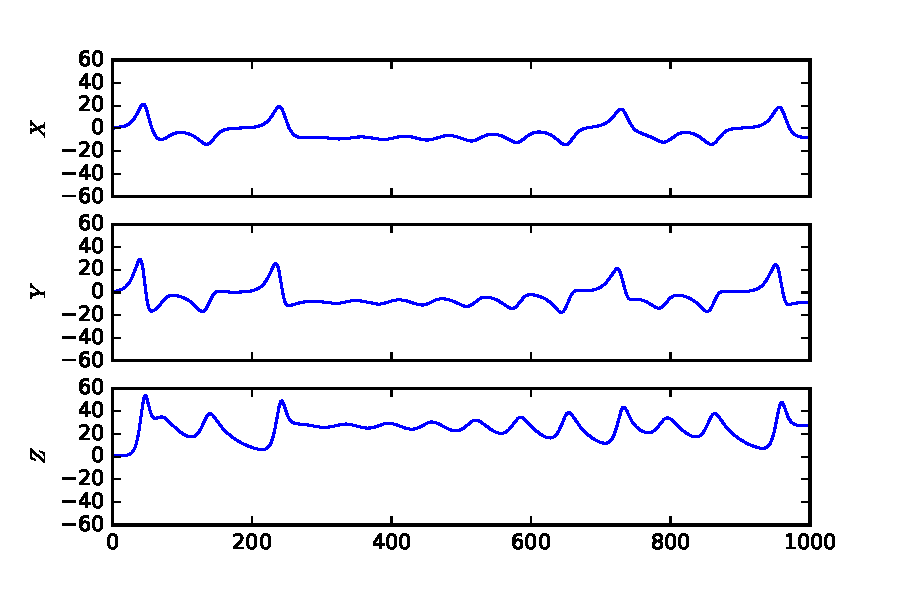
\includegraphics[width=\linewidth]{figures/lorenz_series.pdf}
		\caption{Lorenz system time series}
		\label{fig:lorenz_time_series}
	\end{subfigure}
	\begin{subfigure}{0.45\linewidth}
		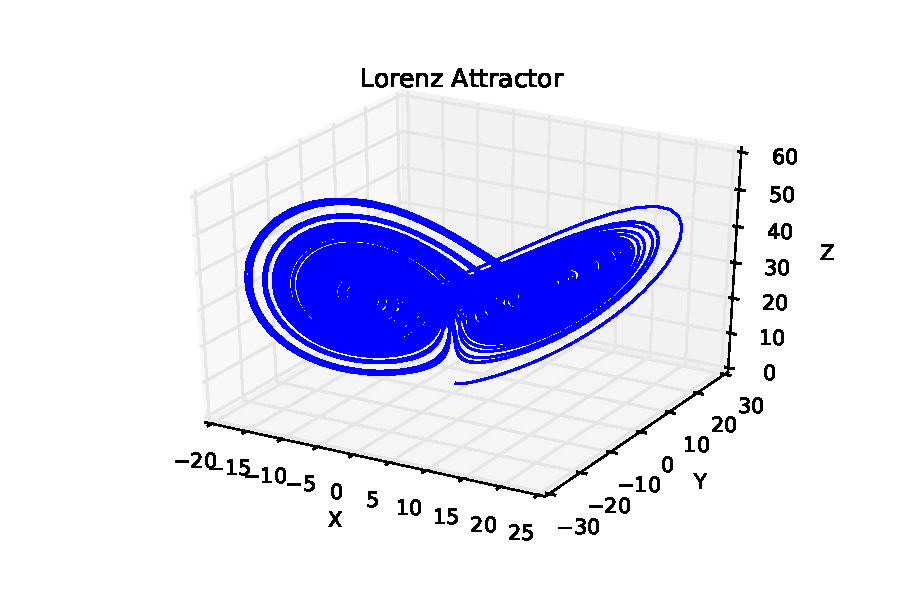
\includegraphics[width=\linewidth]{figures/lorenz.pdf}
		\caption{Lorenz Attractor}
		\label{fig:lorenz_attractor}
	\end{subfigure}
	\caption{A Lorenz system with initial conditions $x=0$, $y=1.0$, $z=1.05$, $\sigma=10$, $\rho=28$, $\beta=2.667$, and time differential of $0.01$. The series represent interlinked components in a system, and the manifold is made up of all the three series combined. The manifold is constructed by mapping the combination of $x$, $y$, and $z$ at each unique time point to a coordinate in an $n$-dimensional space, where $n$ is the number of components---$n=3$ in this case. The resulting mathematical $n$-dimensional object is called a manifold, and can be used to describe the state of the system in terms of complexity, flux, and stability. In this given example, it can be seen that the system gravitates towards two main "loops", and therefore the system is \textit{attracted} to those points in the three dimensional space.}
	\label{fig:lorenz}
\end{figure}

\subsection{Shadow Manifolds}
A shadow manifold of time series $\omega$ is an $E$ dimensional reconstruction of $E$ delayed signals of $\omega$. For example, if our $\omega$ variable is actually the \textit{sin} function, then to construct $E$ delayed signals of $\omega$ we would calculate

\begin{align*}
	\omega_1(t) &= sin(t) \\
	\omega_2(t) &= sin(t-1) \\
	\omega_3(t) &= sin(t-2) \\
	\vdots& \\
	\omega_E(t) &= sin(t-(E-1)) \\
\end{align*}

and then to construct a shadow manifold of $\omega$ we would construct a manifold of $\omega_1$, $\omega_2$, $\dots$ , $\omega_E$ (Fig. \ref{fig:sin_shadow_manifold}). Since the scalar by $1$ increment seems too general, the signals are delayed by multiples of $\tau$, where $\tau$ is approximated by field knowledge or mathematical analysis. Therefore, the formal way to describe shadow manifolds is that they are signals delayed by a  scalar multiple of $E\tau$ such that shadow the manifold of $\omega$, $M_{\omega}$, is described as 
\begin{align*}
	M_{\omega} &= f\Big(\omega_1(t), \omega_2(t), \omega_3(t), \dots, \omega_E(t)\Big)\\
	&= f\Big(\omega(t), \omega(t-\tau), \omega(t-2\tau), \dots, \omega(t-(E-1)\tau)\Big)
\end{align*}


\begin{figure}
	\centering
	\begin{subfigure}{0.45\textwidth}
		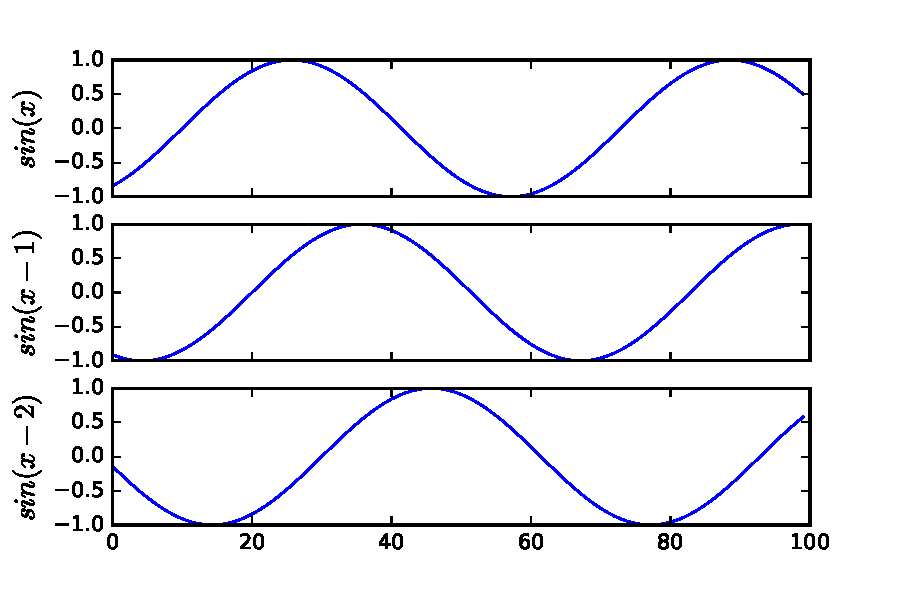
\includegraphics[width=\linewidth]{figures/sin_delayed_signal.pdf}
	\end{subfigure}
	\begin{subfigure}{0.45\linewidth}
		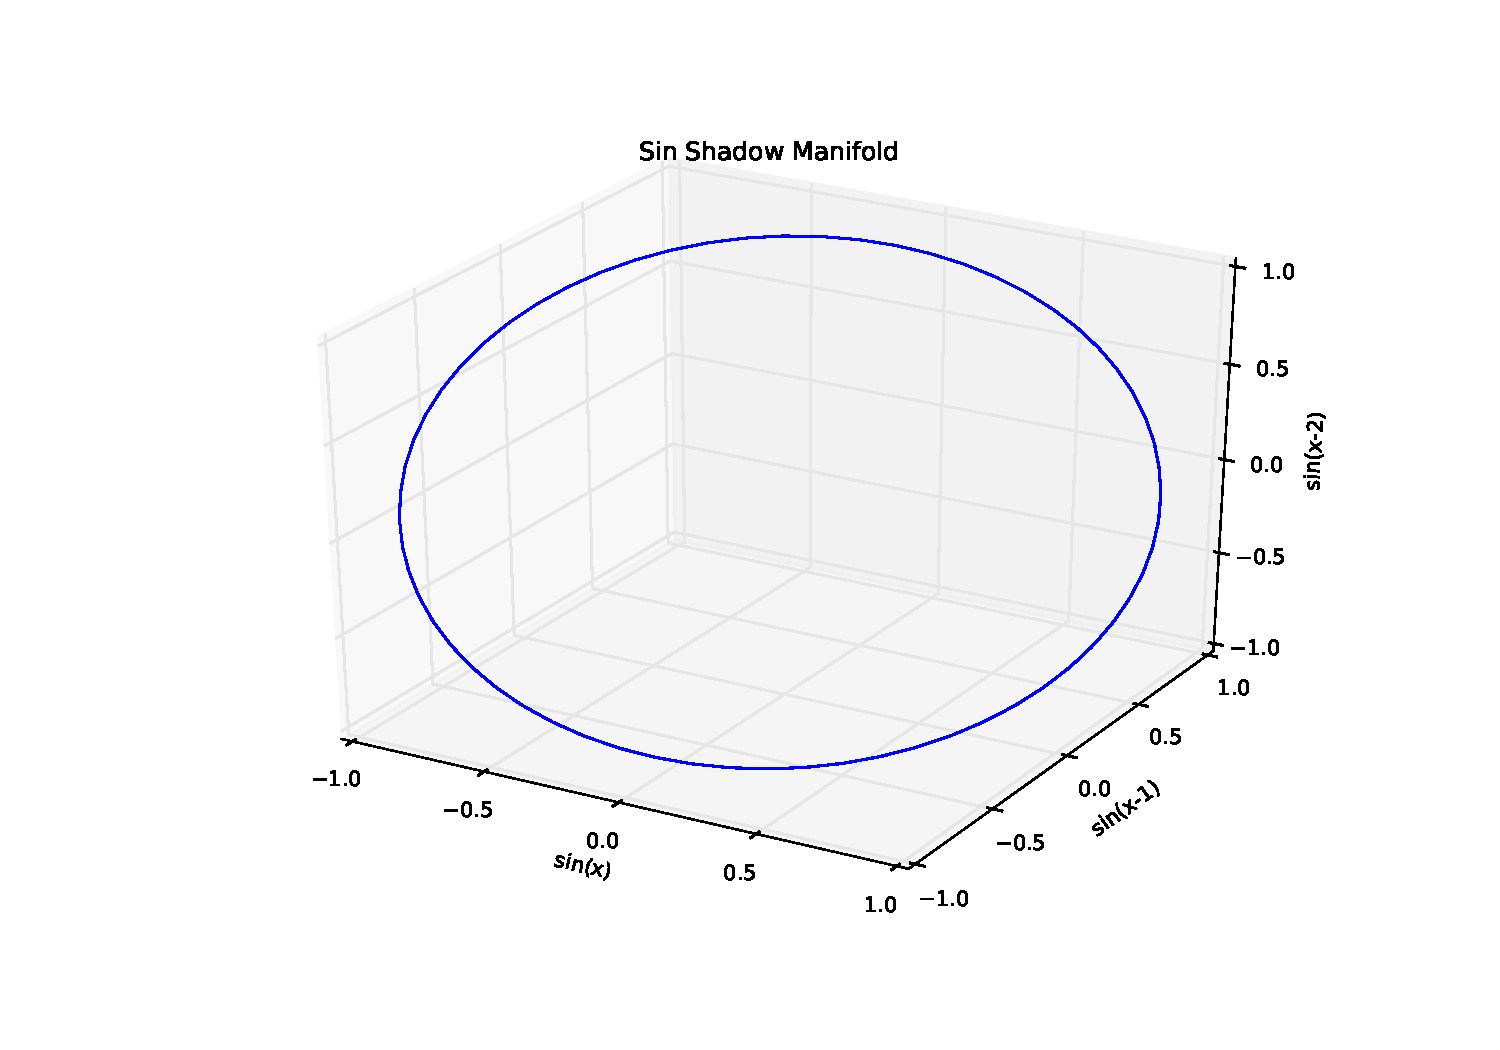
\includegraphics[width=\linewidth]{figures/sin_shadow_manifold.pdf}
	\end{subfigure}
	\caption{A shadow manifold of a simple sin function. The delayed signals are created by delaying the series by a scalar constant $\tau$ (in this case $\tau=1$ and $E=3$ so the function is delayed by $1,2,3$). From these delayed signals, a manifold is constructed by mapping each time point of all the delayed signals to an $E$-dimensional manifold called a shadow manifold.}
	\label{fig:sin_shadow_manifold}
\end{figure}


By using a theorem called Takens' embedding theorem, it can be shown that each shadow manifold of a variable is a projection of the dynamic system's manifold, $M$, that preserves the topology of $M$ \cite{Dixon1999,Deyle2011,Takens1981}. For example, in a dynamic system like the Lorenz Attractor where the dynamics of each variable is affected by the other variables in the system, it can be said that each variable subscribes to the overall dynamic of the system. Therefore, the state of one variable could be used to infer the state of another variable if they are dynamically linked. A visual demonstration of this can be seen in Figure \ref{fig:lorenz_topology} where the shadow manifold of each of the variables in the Lorenz system maintains part of the topology of the original whole system. This important property of shadow manifolds imply that there is a one-to-one relationship between a shadow manifold and the original system manifold. More importantly, this also implies that there is a one-to-one relationship between the shadow manifold of one variable and each of the other shadow manifolds in the system. Therefore, the relationship between each shadow manifold is strong. A great demonstration of this concept can be viewed in the online (Science) version of the original paper by Sugihara \cite{Sugihara2012} where a video is present to elegantly describe this concept (for ease of access, the reader can also refer to a youtube video called "Takens' theorem in action for the Lorenz chaotic attractor" \cite{TakensYoutube2012}). 

\begin{figure}
	\centering
	\begin{subfigure}{0.30\textwidth}
		\centering
		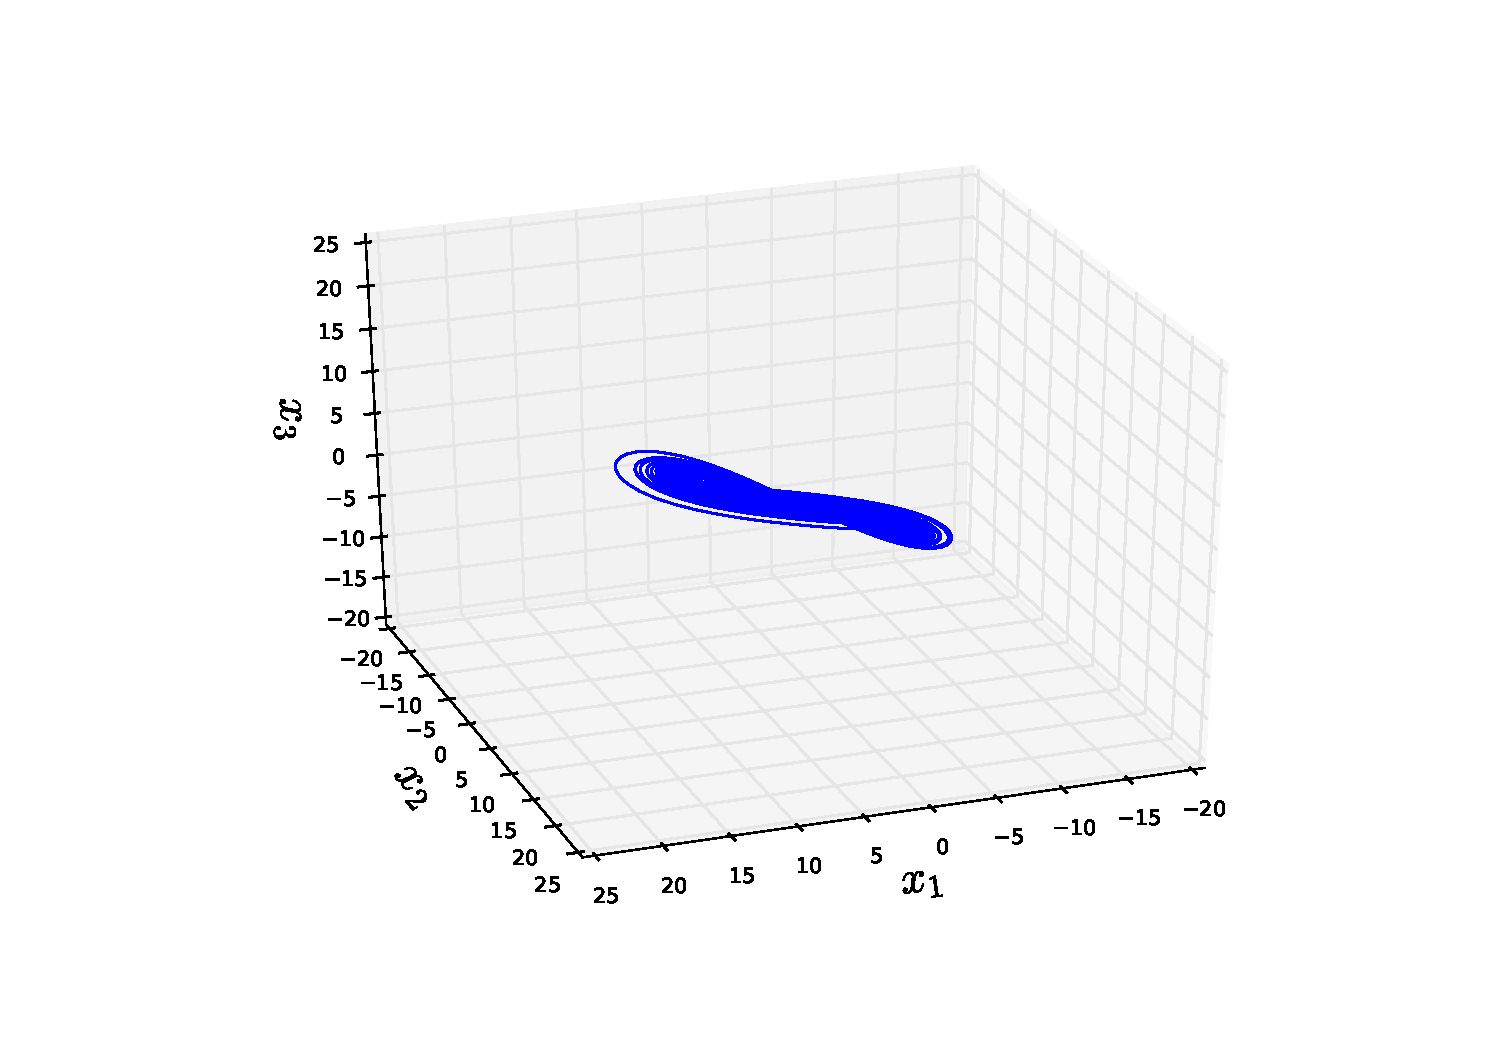
\includegraphics[width=\linewidth]{figures/shadow_manifold_x.pdf}
	\end{subfigure}
	\begin{subfigure}{0.30\textwidth}
		\centering
		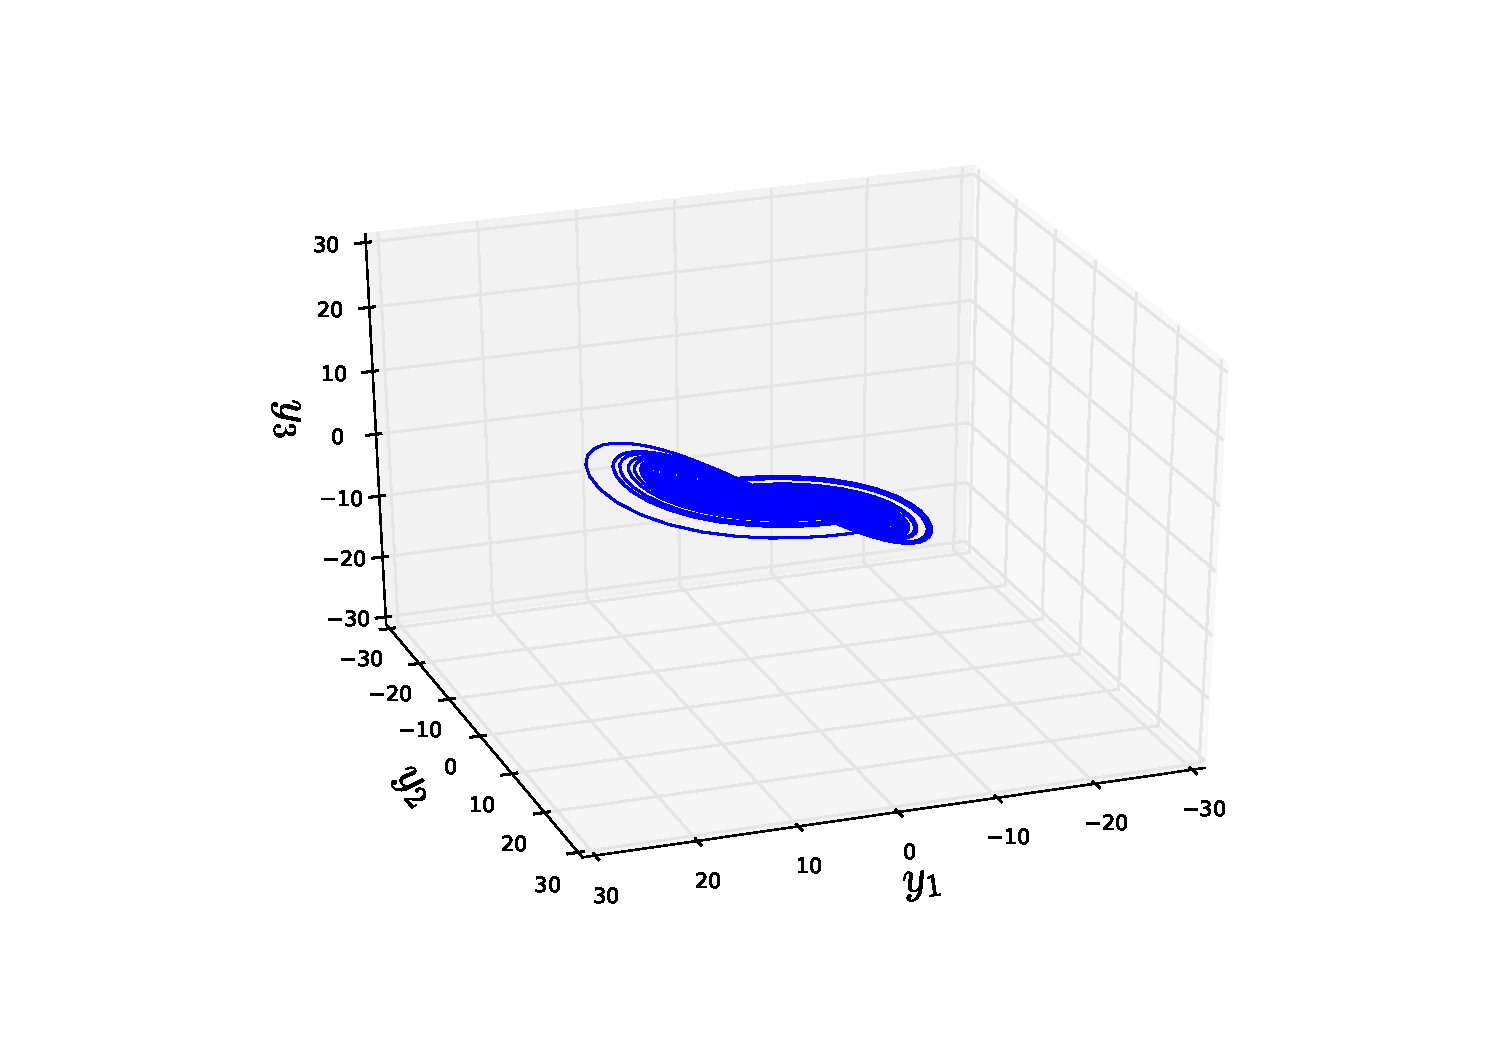
\includegraphics[width=\linewidth]{figures/shadow_manifold_y.pdf}
	\end{subfigure}
	\begin{subfigure}{0.30\textwidth}
		\centering
		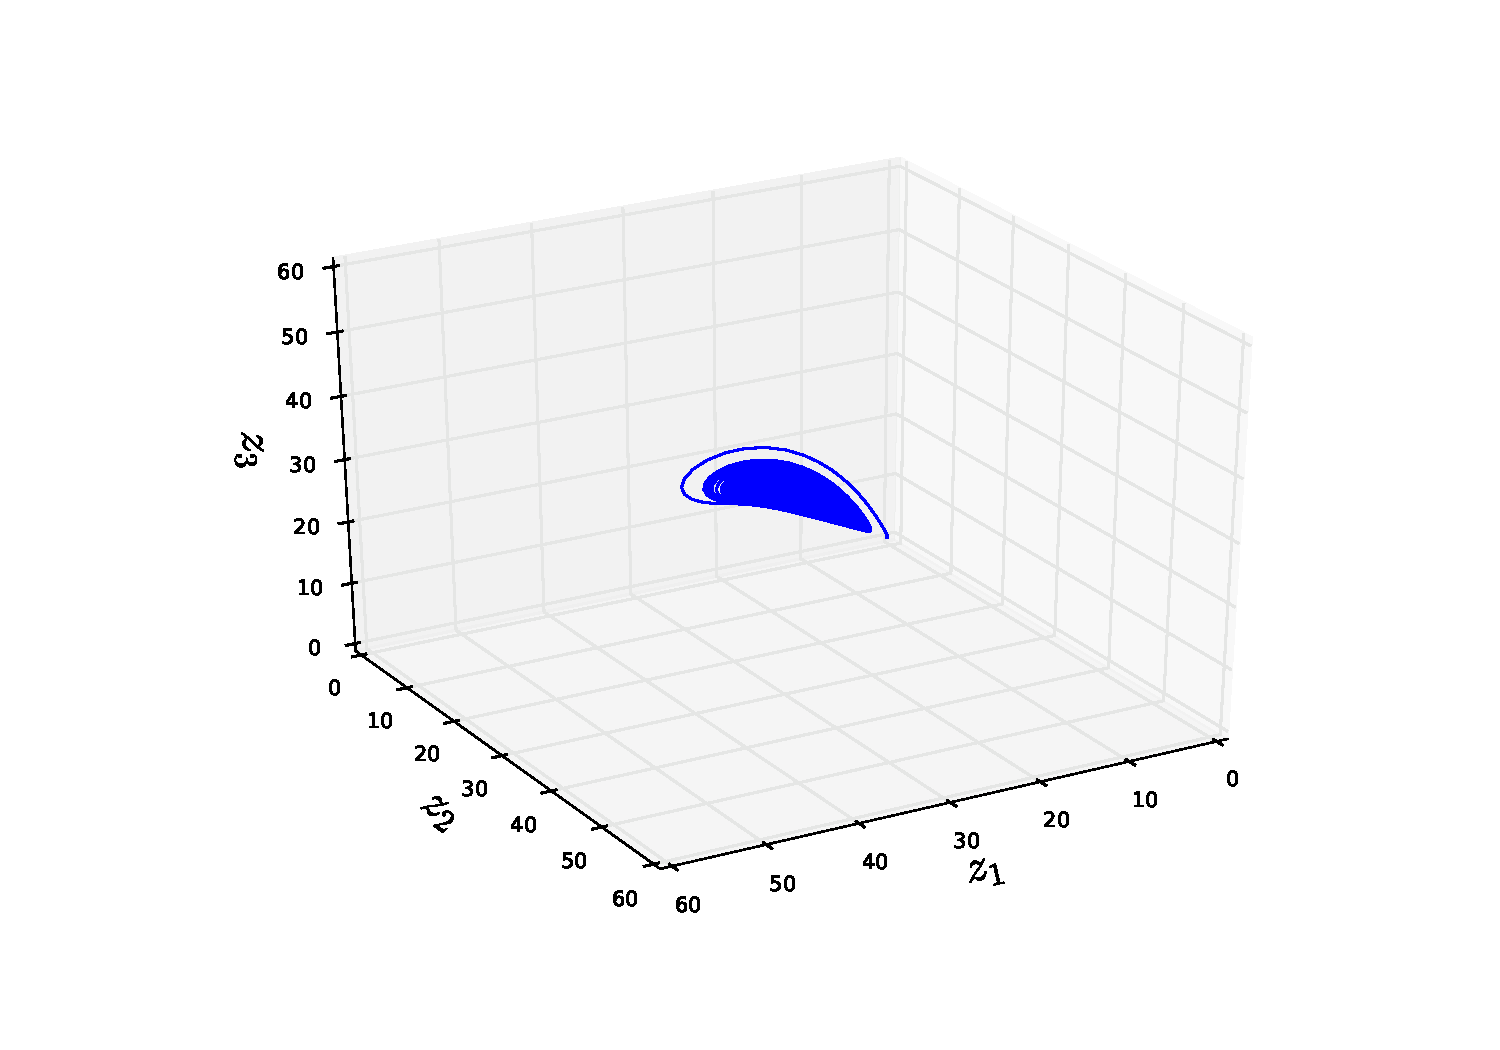
\includegraphics[width=\linewidth]{figures/shadow_manifold_z.pdf}
	\end{subfigure}
	\caption{The shadow manifolds of variables $x$, $y$, and $z$ in the Lorenz system. Each of the shadow manifolds retains part of the topology of the original system, as proven by Takens' theorem \cite{Takens1981}.}
	\label{fig:lorenz_topology}
\end{figure}

\subsection{Convergent Cross Mapping}
Using the mentioned dynamic relationship between shadow manifolds, the Sugihara Causality is calculated as the distance between points of similar time point on each shadow manifold. For variables $x$ and $y$, the causality at time $t$ is calculated as a measure of the time difference between closest neighbors of $y_t$. This concept is called cross-mapping, and is illustrated in the supplemental materials on the original paper, and the youtube video referred to previously \cite{Sugihara2012, TakensYoutube2012}. The last portion of the Sugihara model is the Convergent in Convergent Cross Mapping, which refers to the convergence of the causality value (cross mapping score) when the library of reference points in $x$ and $y$, $L$, is considered. The library $L$ simply refers to the specific range of $x$ and $y$ values to be used in the cross mapping calculation. For example, $L$ could be 20, which means only 20 time-synced data point observations of $x$ and $y$ are taken into consideration, or it could be $100$, which means 100 $x$ and $y$ variables are considered. The Sugihara model expects for a causal relationship to \textit{converge} to a value as $L$ increases. This implies that $L$ needs to be sufficiently large to allow an observation of convergence. This convergence is the test used to determine Sugihara Causality, named after its author who describes it as a required but not complete definition of causality \cite{Sugihara2012}. This approach is the first step towards more general and applicable causality models since Granger Causality. Since the introduction of Convergent Cross Mapping, it has been shown to be successfully predictive in biological \cite{Deyle16042013,Wang2014,Sugihara2012,Mcbride2015,Nes2015} and cosmological \cite{Tsonis2015} applications while showing weaknesses in others \cite{Mccracken2014}. 

\subsection{Growth of CCM}
Extensions to and amalgamations of the CCM model are beginning to surface in literature. Clark \textit{et al.} proposed an extension to CCM that relies on measuring the smoothness of the mapping (also called flow) function $\phi$, thereby reducing the $L$ length requirement\cite{Clark2015}.  Wismüller \textit{et al.} proposed a Mutual Connectivity Analysis framework for the "analysis and visualization of non-linear functional connectivity in the human brain from resting state functional MRI" \cite{wismuller2014} which relies heavily on CCM. Tajima \textit{\textit{et al.}} use the fundamental idea of state space reconstruction to find two measures. The first is \textit{Complexity} which is the best embedding dimension for a certain signal (embedding dimension at which the cross mapping is saturated). The second is \textit{directionality}, the difference in cross map skill or embeddedness between two a pair of signals. With those two measures, they show that the brain exhibits different complexities during conscious and unconscious states. Here, we explore the application of CCM in estimating the causality between neuronal regions by constructing a network of pairwise causality. We then analyze features of such networks during normal and epileptic seizure periods, and use this in conjunction with machine learning to observe if Sugihara Causality can unearth modes of communication in the brain.

